\section{Language background}\label{sec:LanBac}
Amarasi is a variety of Meto.
Meto, also known as Uab Meto, Dawan(ese), Timorese or Atoni,\footnote{
		In earlier works I referred to this language cluster as Uab Meto.
		In Amarasi \ve{uab metoʔ} can be glossed as `dry/indigenous speech'.
		However, not all Meto speaking areas use \ve{uab} for `speech'.
		Thus, in Amfo{\Q}an `speech' is \ve{aguab} while
		in some other areas, such as Timaus, it is \ve{molok}.
		Use of \emph{Meto} alone as the name of the language cluster
		thus covers more varieties in an emic manner.
		It also matches native use in which \ve{metoʔ} alone
		can refer to the language.
		Such use is seen in phrases such as
		\ve{iin nahiin metoʔ} `S/he knows (how to speak) Meto'.}
is a cluster of closely related Austronesian languages
and dialects spoken on the western part of the island of Timor;
both in the East Timorese enclave of Oecusse,
as well as in the Indonesian province of Nusa Tenggara Timur.
The location of the Meto cluster is shown in \frf{fig:LanGroTim}
along with other languages of Timor.
The identity and location of languages in Timor-Leste
in \frf{fig:LanGroTim} is mainly based on \cite{wiklwi15}.

\begin{figure}[h]
	\caption{Language groups of Timor}\label{fig:LanGroTim}
	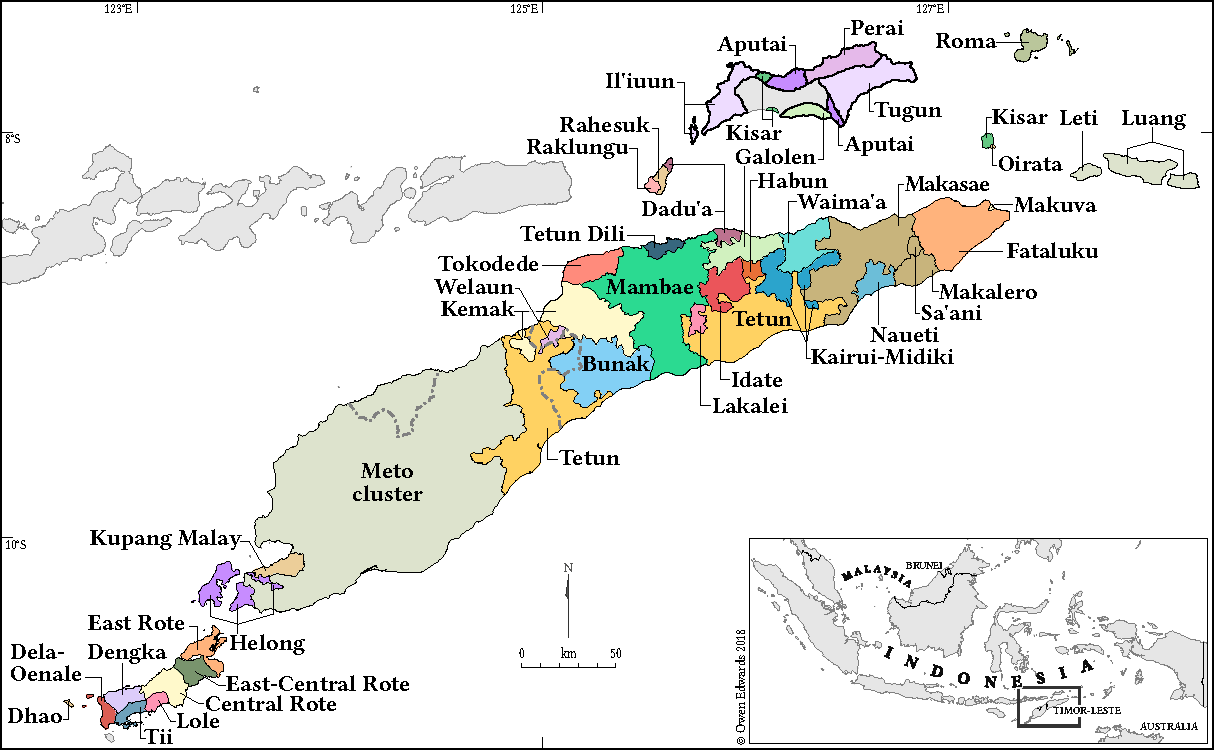
\includegraphics[width=\columnwidth]{TimorLanguages-LinLib.pdf}
\end{figure}

Meto speakers think of their speech as a single language
and call it \it{(uab) metoʔ}, \it{(bahasa) timor}
or occasionally \it{(bahasa) dawan}.
Speakers also recognize more than a dozen named varieties of Meto.
These varieties themselves have named dialects,
with further differences found between different villages and hamlets of a single dialect.
A map of self-identified Meto varieties is given in \frf{fig:SelIdeVarUabMeto}.

\begin{figure}[ht]
	\caption{Self-identified varieties of Meto}\label{fig:SelIdeVarUabMeto}
	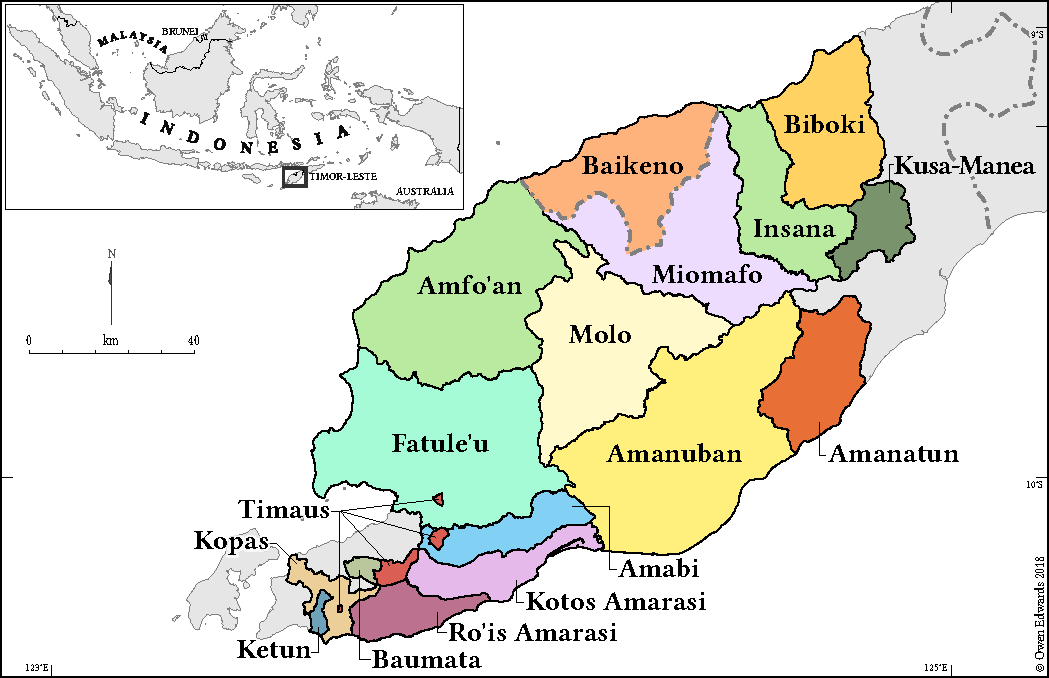
\includegraphics[width=\columnwidth]{Metos-LinLib.pdf}
\end{figure}

The borders of the self-identified varieties of Meto shown in \frf{fig:SelIdeVarUabMeto}
match closely the borders of the pre-colonial political kingdoms of western Timor.\footnote{
		The main exceptions are Kusa-Manea, which was
		part of the Tetun speaking Wehali kingdom,
		as well as Timaus, Baumata, Kopas, and Ketun, which all
		appear to be the result of migrations from more northerly areas.}
The extent to which these boundaries follow linguistic differences is unknown.
In reality, the Meto cluster is a complex language/dialect chain,
and is comparable to more well known cases such as the German chain or the Romance chain.
The nature and extent of variation among Meto varieties has not been fully studied.
Phonological, lexical, semantic, and grammatical diversity is not insignificant
and speakers frequently report difficulty communicating with speakers of other varieties.
As a result, Meto speakers of different varieties often
use a mixture of Meto and Indonesian/Kupang Malay in order to communicate.

\subsection{Affiliation}
Within Austronesian, Meto belongs to the Malayo-Polynesian subgroup
which includes all Austronesian languages outside of Taiwan.
It would further belong to Central Malayo-Polynesian
within Central-Eastern Malayo-Polynesian
\citep{bl81,bl93,bl09b} but the extent
to which these constitute valid
linguistic subgroups is contested \citep{ro95,ad05,dogr08}.

Closer to home, the nearest genealogical relative of Meto is the Rote cluster
spoken on the island of Rote just to the south-west of Timor.
Based on shared sound changes, Rote-Meto can be placed in a Timor-Babar
subgroup which contains the Austronesian languages of Timor and south-west Maluku
(from Babar island to Wetar island), though excluding
Mambae, Tokodede, Welaun, and Kemak which
form a Central Timor subgroup \citep{ed18d,ed19}.

While Meto is demonstrably Austronesian,
it has strong influence from at least one -- probably more --
pre-Austronesian languages of the region \citep{ed16c,ed18b}.
This substrate is reflected at all levels of the language:
lexicon, phonology, morphology, and syntax.

Typologically, Meto fits well in the Melanesian linguistic area with four to five
of the six properties identified by \cite{sc15} as constituting this area.
The only property of linguistic Melanesia which Meto unambiguously lacks
is that of having complex numerals below ten.
Apart from this Meto has genitive-noun order,
absence of velar nasal /ŋ/, noun-numeral order
and possessive classification,
all of which are typical of linguistic Melanesia.

Another property of linguistic Melanesia is verb-negator order.
Regarding this property, most varieties of Meto
for which data is available have double negation
with \ve{ka=} occurring before the verb and \ve{=fa} after the verb.
However, Ro{\Q}is Amarasi has post-verbal \ve{=maeʔ}
while Amfo{\Q}an only has pre-verbal \ve{ka=}.

While Meto fits well within linguistic Melanesia,
it is, based on current understanding,
only a peripheral member of linguistic Wallacea as identified by \cite{sc15}.
\citeauthor{sc15} gives four properties of linguistic
Wallacea: cognates of \su{\#}muku `banana', neuter gender,
semantic alignment, and synchronic metathesis.
Of these, Meto only has synchronic metathesis.

\subsection{Amarasi}\label{sec:Amarasi}
Amarasi is spoken towards the south-west end of the Meto speech area.
One salient feature which sets Amarasi apart from most other Meto
varieties is the liquid /r/ instead of /l/;
most Meto varieties have only a single liquid.\footnote{
		Amabi also has /r/ instead of /l/ as does
		Kusa-Manea, though /l/ occurs in many Tetun loanwords in Kusa-Manea.
		Timaus has both /l/ and /r/ due to a *{\j} > /r/ sound change.}

Amarasi speakers identify three Amarasi dialects: Kotos, Ro{\Q}is, and Tais Nonof.
Current data indicates that Tais Nonof is a label for the speech of
those living along the coast of the Amarasi area,
including those whose speech is most similar to Kotos Amarasi
and those whose speech is most similar to Ro{\Q}is Amarasi.
Amarasi speakers also report that the Amabi variety of Meto
is very similar to their own speech with minor lexical differences.

Differences between Kotos Amarasi and Ro{\Q}is Amarasi
include different functors (grammatical morphemes),
lexicon, phonotactics, as well as having undergone different sound changes.
A number of functors in Ro{\Q}is and Kotos Amarasi
are shown in Table \ref{tab:DifKotRoqFun}
as a sample of the divergence between these two lects.

\begin{table}[h]
	\caption{Different Kotos and Ro{\Q}is functors}\label{tab:DifKotRoqFun}
		\begin{tabular}{lll|lll}
		\lsptoprule
				Kotos 		&Ro{\Q}is 			&gloss		&Kotos 			&Ro{\Q}is 	&gloss	\\ \midrule
				\ve{he}		&\ve{nu}				&{\he}		&\ve{ia}		&\ve{ai}		&{\ia}	\\
				\ve{reʔ}	&\ve{heʔ}				&{\req} 	&\ve{nee}		&\ve{nae}		&{\nee} \\
				\ve{ka={\ldots}=fa}
									&\ve{maeʔ}			&{\kaah}	&\ve{iin}		&\ve{hiin}		&{\iin}	\\
				\ve{on}		&\ve{en}				&{\on}		&\ve{=een}	&\ve{=heen}	&{\een} \\
				\ve{n-bi}	&\ve{n-biʔaak}	&{\bi}		&\ve{nai}		&\ve{neu}		&already \\
				\ve{et}		&\ve{ek/et}			&{\et}		&\ve{u-}		&\ve{ku-}		&{\qu}	\\
				\ve{n-ak}	&\ve{tauʔ/n-ak}	&{\ak}		&\ve{-k}		&\ve{-r}		&\tsc{3pl.gen}\\
				\ve{n-eu}	&\ve{n-uu}			&{\eu}		&\ve{a-{\ldots}-t}&\ve{ka-{\ldots}-t}&\tsc{\at}\\
			\lspbottomrule
		\end{tabular}
\end{table}

In fact, looking only at linguistic structures
and shared sound changes, Kotos Amarasi is more closely
related to other varieties of Meto than it is to Ro{\Q}is Amarasi.
Nonetheless, speakers of Kotos and Ro{\Q}is
self-identify their speech as more similar to one another
than to other Meto varieties.
They frequently interact together
and both share a common history as members of the Amarasi kingdom.
Thus, from a socio-historical perspective,
Kotos and Ro{\Q}is can be considered
``dialects'' of a single language.\footnote{
	Kotos and Ro{\Q}is speakers perceive their speech
	as closer to one another based on salient commonalities
	not found in nearby varieties of Meto.
	Such commonalities include /r/ instead of /l/ and
	lexical items, such as \ve{koʔu}
	`big' instead of \ve{ʔnaek}, or
	\ve{n-kono} `keep going' instead of \ve{n-fini}.}

Data from Kotos Amarasi forms the basis of this book.
I present Ro{\Q}is Amarasi data at various points when it bears on the analysis
of Kotos Amarasi and/or differs in important respects.
My Kotos data comes mostly from the hamlet \emph{(kampung)} Koro{\Q}oto,
in the modern village \emph{(desa)} Nekmese{\Q}.
My Ro{\Q}is data comes from the hamlet
of Suit in the village of Buraen, as well as the hamlets
of Batuna and Ruanrete in the village of Tunbaun.
The locations of these villages within the Amarasi
speech area are shown in \frf{fig:LocNekBurTun}.

\begin{figure}[ht]
	\caption{Locations of Nekmese{\Q}, Buraen, and Tunbaun}\label{fig:LocNekBurTun}
	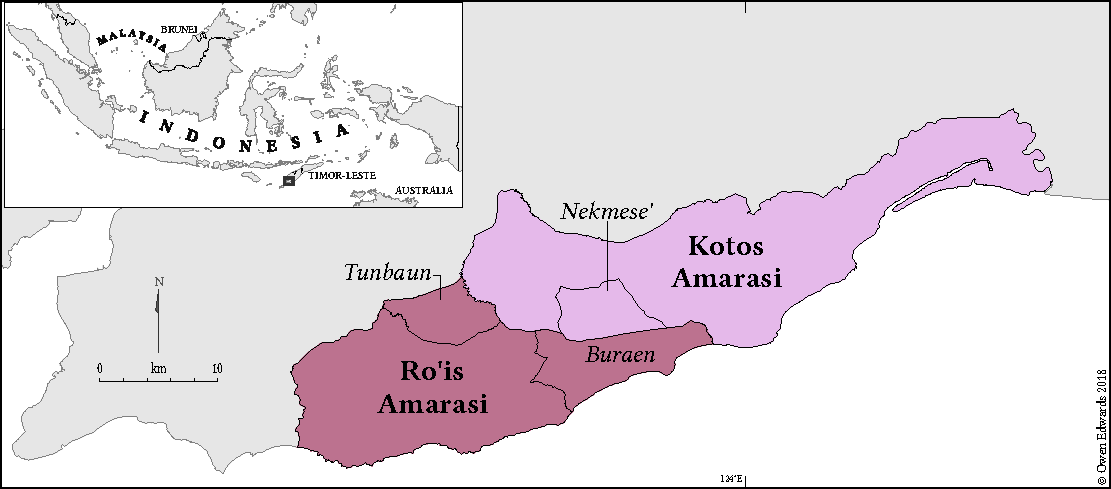
\includegraphics[width=\columnwidth]{Amarasis-LinLib.pdf}
\end{figure}

From 1968--1975 west Timor underwent an administrative restructure
with the creation of the administrative units of districts
(\emph{kecamatan}) and villages (\emph{desa}).
In Amarasi 60 hamlets were amalgamated into 23 villages.
In parts of Amarasi this amalgamation was also accompanied by the 
physical relocation of traditional hamlets in order to allow
for a more efficient development of infrastructure and delivery of services.

Nekmese{\Q} -- data from which forms the core of this work --
was created by the amalgamation of four hamlets:
Koro{\Q}oto, Fo{\Q}asa{\Q}, Tuamese{\Q} and Naet.
These hamlets still exist as \emph{dusun}
(the administrative level below \emph{desa})
and form the basis of the parishes of the dominant
Christian denomination in the village
(the protestant GMIT church\footnote{
		GMIT is an acronym of \emph{Gereja Masehi Injili di Timor};
		for which the official translation is `The Evangelical Protestant Church of Timor'.
		There are four GMIT parishes in Nekmese{\Q}:
		one serving Koro{\Q}oto, one for Fo{\Q}asa{\Q} and Tuamese{\Q}, and two for Naet.})
People also maintain their gardens and fields in the vicinity of the old hamlets.\footnote{
		Inhabitants of Koro{\Q}oto have moved the furthest,
		with \emph{desa} Nekmese{\Q} being located close to the original locations
		of Fo{\Q}asa{\Q} and Tuamese{\Q}.
		The inhabitants of Naet have moved from their original location
		towards Nekmese{\Q}, but Naet remains dislocated from the rest of Nekmese{\Q}.
		The inhabitants of Naet speak the Tais Nonof variety of Amarasi.}

Despite the administrative and physical restructure of 1968--1975,
the traditional hamlets of Nekmese{\Q} are alive and well as distinct social and linguistic units.
A summary of the speech variety which is the focus of this work is given in \qf{ex:SpeVar} below.
Unless explicitly labelled otherwise,
all data is Kotos Amarasi from the hamlet of Koro{\Q}oto.

\begin{exe}
	\ex{
		\begin{xlist}
			\ex{Language: \emph{Meto}}
			\ex{Variety: \emph{Amarasi}}
			\ex{Dialect: \emph{Kotos}}
			\ex{Hamlet: \emph{Koro{\Q}oto}}
		\end{xlist}
	}\label{ex:SpeVar}
\end{exe}
